\chapter{Experimentación.}\label{cap:capitulo7}


\section{Interfaz de experimentación.}


\section{Flexibilidad y posibilidades.}


\section{Eficiencia}

Recordemos que, aunque no se restringía un tamaño al escenario, se estima como tamaño máximo un escenario de 64x64 tiles. Aún así, para estresar el algoritmo, se han elaborado mapas con tamaños mayores. Por ejemplo, en uno de ellos el tamaño de habitación de 20x20, y en el mejor caso, con habitaciones de este tamaño cuadradas, podríamos tener 9 en un mapa de 64x64, pero veremos tiempos bastante buenos con una generación de este tipo hasta para escenarios de 30 habitaciones.

Como no se ha implementado en móvil, se ha considerado que un tiempo es bueno, cuando es menor de un segundo. Si es menor de dos segundos, también se considerará como aceptable. Aún así, habría que hacer una prueba real, que debido a que Java es la plataforma de elección para el desarrollo a Android, no sería complejo. En un caso real de un juego de móvil además, se presupone menor complejidad debido al sistema donde se ejecuta, y se puede entender que un tiempo aceptable de espera a la generación es hasta 10 segundos, y en esto se fundamenta la aceptación de menor de dos segundos como solución buena.

Destacar que las mediciones realizadas para comprobar el impacto de algunos parámetros se han usado sin tener en cuenta los demás. Al final, podremos ver una medición realizada sobre una configuración que se ha conseguido con tiempos muy buenos y calidad notable.

Las pruebas se han realizado en un portátil HP Compaq Presario V6000 con las siguientes características:

\begin{center}
	\begin{tabular}{ | c | c | }
\hline
Modelo procesador & AMD Athlon 64 X2 \\ 
Núcleos procesador & 2 (1 en uso) \\
Velocidad procesador & 1.7 Ghz \\
Caché procesador & 512 KB L2 \\
Memoria RAM & 1 GB \\
\hline
	\end{tabular}
\end{center}


\subsection{Impacto del factor divisor de movimientos}

Como se comentó anteriormente (ENLACE A ESTO), el factor de divisor de movimientos permite elegir un subconjunto de todos los movimientos posibles para cada paso de la generación.

Se han realizado pruebas con la configuración para el resto de parámetros como se indica en la tabla~\ref{table:cfgdpediv}, modificando el parámetro de divisor de movimientos para los valores 0.75, 0.85 y 0.95.

\begin{table}[H]
\begin{center}
	\begin{tabular}{ | c | c | }
\hline
 		Property & Value \\ \hline
DoorGenType & ALL \\ 
SolverType & BestSearch \\ 
CacheType & NO CACHE \\ 
\hline
	\end{tabular}
\end{center}
\caption{Configuración para divisor de movimientos}
\label{table:cfgdpediv}
\end{table}

\begin{table}[H]
\begin{center}
	\begin{tabular}{ | c | c | c | c | c | c | c | }
\hline
Tam. habs. & Modelos & Inst./modelo & Total habs. & 0.75f & 0.85f & 0.95f\\ \hline 
10 & 2 & 20 & 40 & 0.1763 & 0.1967 & 0.3667 \\ 
10 & 2 & 30 & 60 & 0.4945 & 0.6254 & 1.4392 \\ 
10 & 4 & 20 & 80 & 1.2336 & 1.6429 & 4.0735 \\ 
10 & 4 & 30 & 120 & 4.8805 & 6.6694 & 18.1853 \\ 
\hline
	\end{tabular}
\end{center}
\caption{Influencia del divisor de movimientos}
\label{table:dpediv}
\end{table}


\begin{figure}[H]
\centering
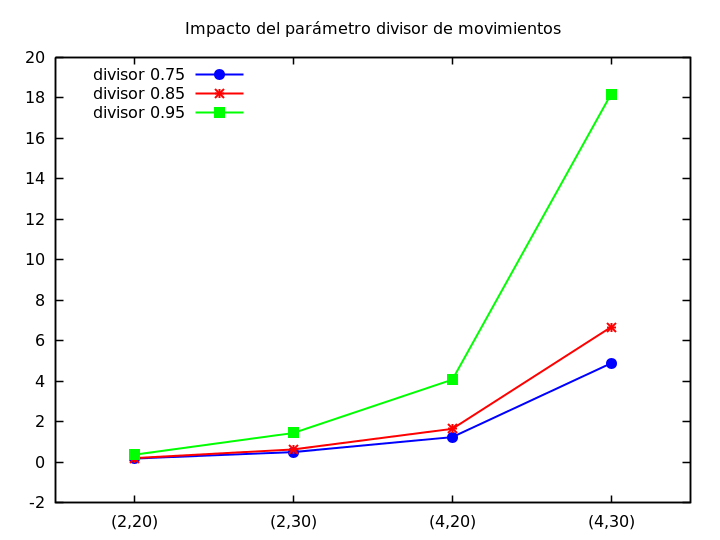
\includegraphics[scale=0.5]{img/dpedivs}
\caption{Gráfica de comparación de parámetro divisor de movimientos
\label{fig:grfdpedivs}}
\end{figure}



\subsection{Impacto de la generación de puertas aleatoria}

\begin{table}[H]
\begin{center}
	\begin{tabular}{ | c | c | }
\hline
 		Property & Value \\ \hline
DoorGenType & RANDOM \\ 
SolverType & BestSearch \\ 
BestSearch DPE Divisor & 1.0 \\ 
CacheType & NO CACHE \\ 
\hline
	\end{tabular}
\end{center}
\caption{Configuración del test de impacto de generación de puertas aleatorias}
\label{table:cfg-randoors}
\end{table}


\begin{table}[H]
\begin{center}
	\begin{tabular}{ | c | c | c | c | c | c | c | }
\hline
Tam. habs. & Modelos & Inst./modelo & Total & 0.8f & 0.6f & 0.4f \\ \hline 
10 & 4 & 8 & 32 & 4.6552 & 3.3017 & 1.7974 \\ 
10 & 4 & 10 & 40 & 9.8173 & 8.2366 & 4.1857 \\ 
10 & 6 & 8 & 48 & 29.2931 & 20.9267 & 15.4530 \\ 
10 & 6 & 10 & 60 & 69.2747 & 57.3447 & 34.6857 \\ 
\hline
	\end{tabular}
\end{center}
\caption{Test de impacto de generación de puertas aleatorias}
\label{table:randoors}
\end{table}


\begin{figure}[H]
\centering
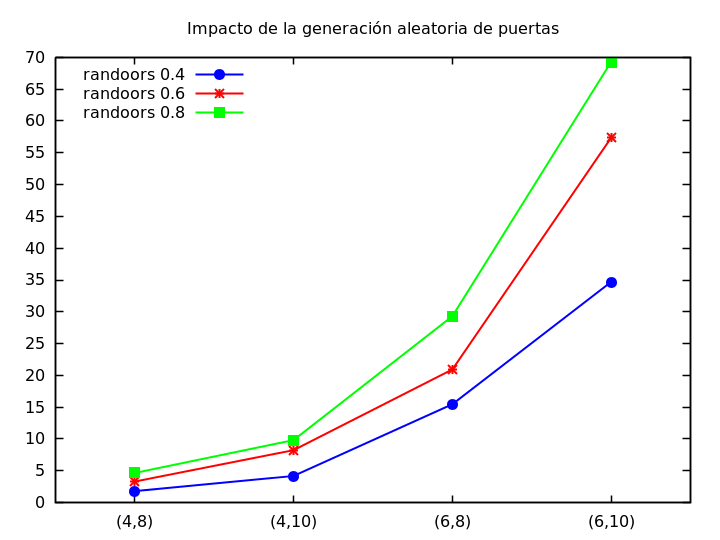
\includegraphics[scale=0.5]{img/randoors}
\caption{Gráfica de comparación de parámetro de generación de puertas aleatorias
\label{fig:grfrandoors}}
\end{figure}


\subsection{Impacto del Caché Refresher}

\begin{table}[H]
\begin{center}
	\begin{tabular}{ | c | c | }
\hline
 		Property & Value \\ \hline
DoorGenType & ALL \\ 
SolverType & BestSearch \\ 
BestSearch DPE Divisor & 1.0 \\ 
CacheType & REFRESHER \\ 
\hline
	\end{tabular}
\end{center}
\caption{Configuración de test de impacto de caché refresher}
\label{table:cfg-refresher}
\end{table}



\begin{table}[H]
\begin{center}
	\begin{tabular}{ | c | c | c | c | c | c | c | c |}
\hline
Tam. habs. & Modelos & Inst./modelo & Total & N=2 & N=5 & N=10 \\ \hline 
6 & 4 & 10 & 40 & 1.3768 & 1.0284 & 0.7653 \\ 
6 & 4 & 15 & 60 & 6.7213 & 5.5230 & 3.4248 \\ 
6 & 6 & 10 & 60 & 8.7300 & 6.7349 & 5.5666 \\ 
6 & 6 & 15 & 90 & 43.7862 & 35.1948 & 26.3091 \\ 
\hline
	\end{tabular}
\end{center}
\caption{Test de impacto de caché refresher}
\label{table:refresher}
\end{table}


\begin{figure}[H]
\centering
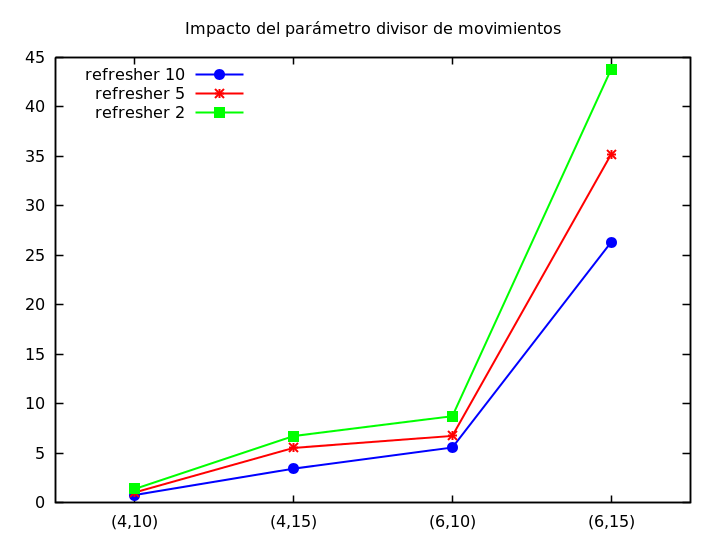
\includegraphics[scale=0.5]{img/refresher}
\caption{Gráfica de comparación de parámetro de caché refresher
\label{fig:grfrefresher}}
\end{figure}



\subsection{Ejemplo optimizado}

\begin{table}[H]
\begin{center}
	\begin{tabular}{ | c | c | }
\hline
 		Property & Value \\ \hline
DoorGenType & RANDOM \\ 
Refresher cache divisor & 10 \\ 
SolverType & BestSearch \\ 
BestSearch DPE Divisor & 0.9 \\ 
CacheType & REFRESHER \\ 
Random doors param & 0.5 \\ 
\hline
	\end{tabular}
\end{center}
\caption{Configuración para test optimizado de tamaño medio}
\label{table:cfg-bsoptmedsamp}
\end{table}

\begin{table}[H]
\begin{center}
	\begin{tabular}{ | c | c | c | c | c | }
\hline
Tam. habs. & Modelos & Instancias/modelo & Total habs. & Tiempo \\ \hline 
10 & 5 & 1 & 5 & 0.0035 \\ 
10 & 5 & 2 & 10 & 0.0127 \\ 
10 & 5 & 3 & 15 & 0.0246 \\ 
10 & 10 & 1 & 10 & 0.0257 \\ 
10 & 10 & 2 & 20 & 0.1216 \\ 
10 & 10 & 3 & 30 & 0.1667 \\ 
10 & 15 & 1 & 15 & 0.1143 \\ 
10 & 15 & 2 & 30 & 0.3776 \\ 
10 & 15 & 3 & 45 & 0.8163 \\ 
\hline
	\end{tabular}
\end{center}
\caption{Test optimizado de tamaño medio}
\label{table:bsoptmedsamp}
\end{table}


\begin{table}[H]
\begin{center}
	\begin{tabular}{ | c | c | }
\hline
 		Property & Value \\ \hline
DoorGenType & RANDOM \\ 
Refresher cache divisor & 10 \\ 
SolverType & BestSearch \\ 
BestSearch DPE Divisor & 0.9 \\ 
CacheType & REFRESHER \\ 
Random doors param & 0.5 \\ 
\hline
	\end{tabular}
\end{center}
\caption{Configuración para test real en dispositivos móviles}
\label{table:cfg-optreal}
\end{table}


\begin{table}[H]
\begin{center}
	\begin{tabular}{ | c | c | c | c | c | }
\hline
Tam. habs. & Modelos & Instancias/modelo & Total habs. & Tiempo \\ \hline 
6 & 5 & 1 & 5 & 0.0007 \\ 
6 & 5 & 2 & 10 & 0.0029 \\ 
6 & 5 & 3 & 15 & 0.0073 \\ 
6 & 5 & 4 & 20 & 0.0168 \\ 
6 & 10 & 1 & 10 & 0.0050 \\ 
6 & 10 & 2 & 20 & 0.0266 \\ 
6 & 10 & 3 & 30 & 0.0679 \\ 
6 & 10 & 4 & 40 & 0.1601 \\ 
6 & 15 & 1 & 15 & 0.0157 \\ 
6 & 15 & 2 & 30 & 0.0905 \\ 
6 & 15 & 3 & 45 & 0.3026 \\ 
6 & 15 & 4 & 60 & 0.6859 \\ 
6 & 20 & 1 & 20 & 0.0398 \\ 
6 & 20 & 2 & 40 & 0.2525 \\ 
6 & 20 & 3 & 60 & 0.7766 \\ 
6 & 20 & 4 & 80 & 2.0803 \\ 
\hline
	\end{tabular}
\end{center}
\caption{Test real en dispositivos móviles}
\label{table:optreal}
\end{table}




\subsection{Comparación ejemplo optimizado}

\begin{table}[H]
\begin{center}
	\begin{tabular}{ | c | c | c | c | }
\hline
Property & NoCache & Always & Opt \\ \hline
DoorGenType & ALL & ALL & RANDOM \\
Random doors param & - & - & 0.5 \\
CacheType & - & ALWAYS & REFRESHER \\
Refresher cache divisor & - & - & 10 \\
SolverType & BestSearch & BestSearch & BestSearch \\
BestSearch DPE Divisor & 1.0 & 1.0 & 0.9 \\
\hline
	\end{tabular}
\end{center}
\caption{Configuración para test de comparación}
\label{table:cfg-comp}
\end{table}


\begin{table}[H]
\begin{center}
	\begin{tabular}{ | c | c | c | c | c | c | c | }
\hline
Tam. h. & Modelos & Inst./modelo & Total & NoCache & Always & Opt \\ \hline 
8 & 4 & 2 & 8 & 0.0333 & 0.0174 & 0.0030 \\ 
8 & 4 & 4 & 16 & 0.2818 & 0.0649 & 0.0123 \\ 
8 & 4 & 6 & 24 & 1.2533 & 0.1949 & 0.0354 \\ 
8 & 4 & 8 & 32 & 3.3727 & 0.4231 & 0.0780 \\ 
8 & 6 & 2 & 12 & 0.1696 & 0.0666 & 0.0107 \\ 
8 & 6 & 4 & 24 & 1.7436 & 0.2856 & 0.0481 \\ 
8 & 6 & 6 & 36 & 8.6428 & 1.0331 & 0.1302 \\ 
8 & 6 & 8 & 48 & 19.8587 & 2.7444 & 0.3155 \\ 
8 & 8 & 2 & 16 & 0.5825 & 0.2523 & 0.0210 \\ 
8 & 8 & 4 & 32 & 7.3917 & 1.1891 & 0.1030 \\ 
8 & 8 & 6 & 48 & 33.7262 & 3.6202 & 0.3438 \\ 
8 & 8 & 8 & 64 & 107.0144 & 9.6228 & 0.8999 \\ 
8 & 10 & 2 & 20 & 1.6964 & 1.0235 & 0.0643 \\
8 & 10 & 4 & 40 & 24.2987 & 3.1605 & 0.2243 \\
8 & 10 & 6 & 60 & 113.6830 & 11.2674 & 0.9700 \\
8 & 10 & 8 & 80 & 417.6313 & 28.2073 & 2.1928 \\
\hline
	\end{tabular}
\end{center}
\caption{Test de comparación}
\label{table:comp}
\end{table}


\begin{figure}[H]
\centering
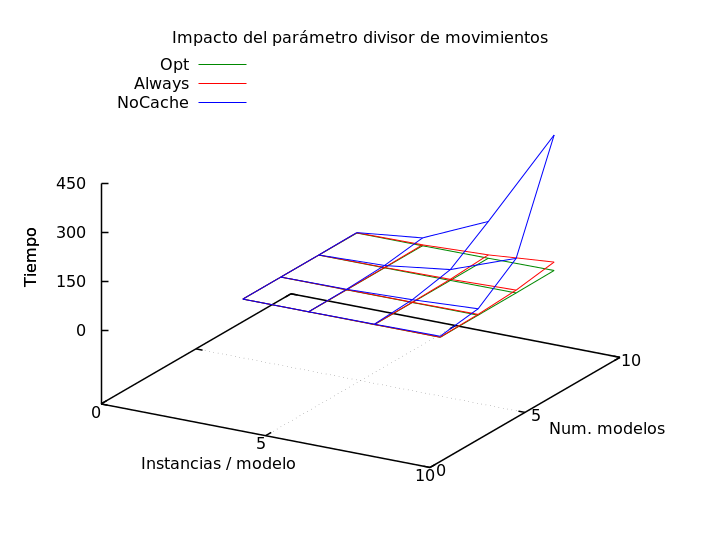
\includegraphics[scale=0.5]{img/comp-all}
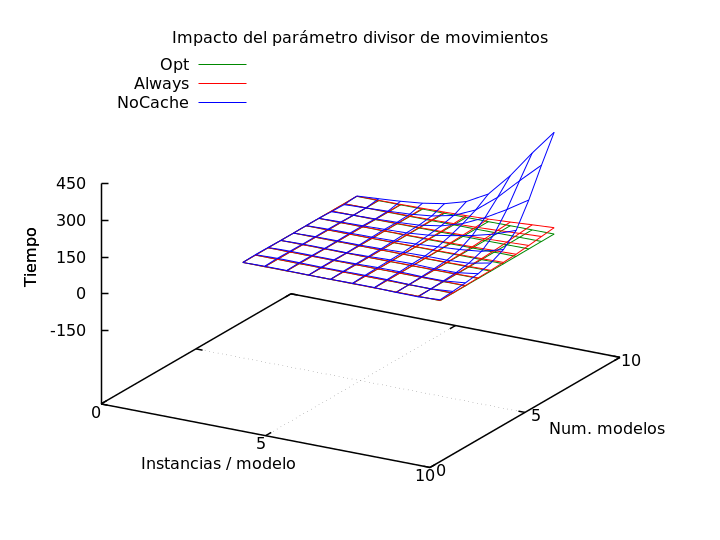
\includegraphics[scale=0.5]{img/comp-all-spl}
\caption{Gráfica de comparación entre AlwaysCache, NoCache y ejemplo optimizado
\label{fig:grfcompall}}
\end{figure}



\begin{figure}[H]
\centering
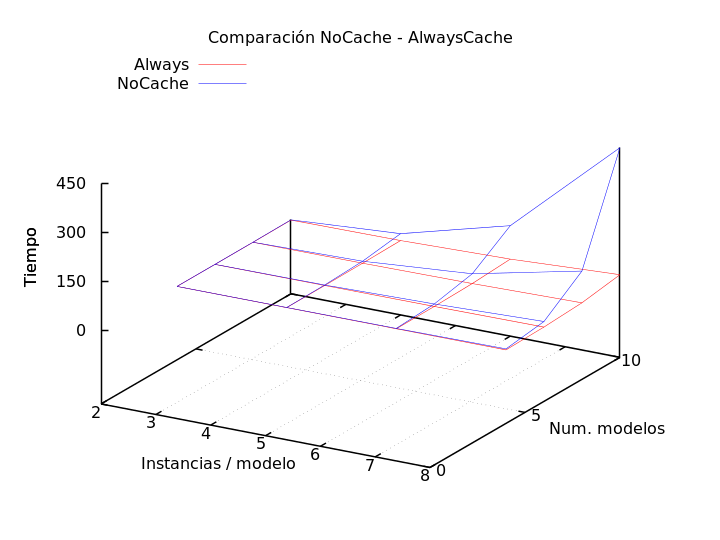
\includegraphics[scale=0.5]{img/comp-nc-alw}
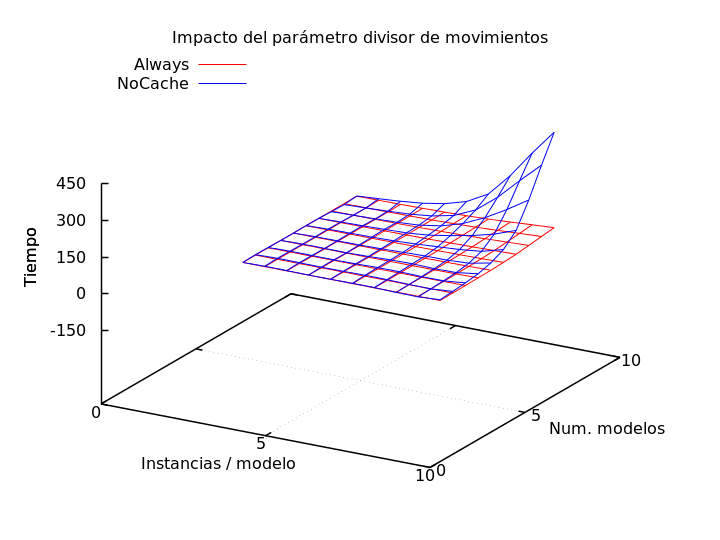
\includegraphics[scale=0.5]{img/comp-nc-alw-spl}
\caption{Gráfica de comparación entre AlwaysCache y NoCache
\label{fig:grfcompall}}
\end{figure}


\begin{figure}[H]
\centering
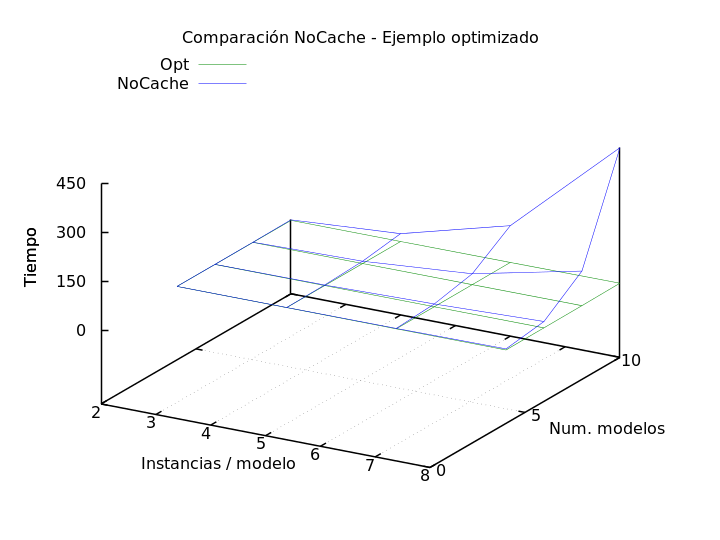
\includegraphics[scale=0.5]{img/comp-nc-opt}
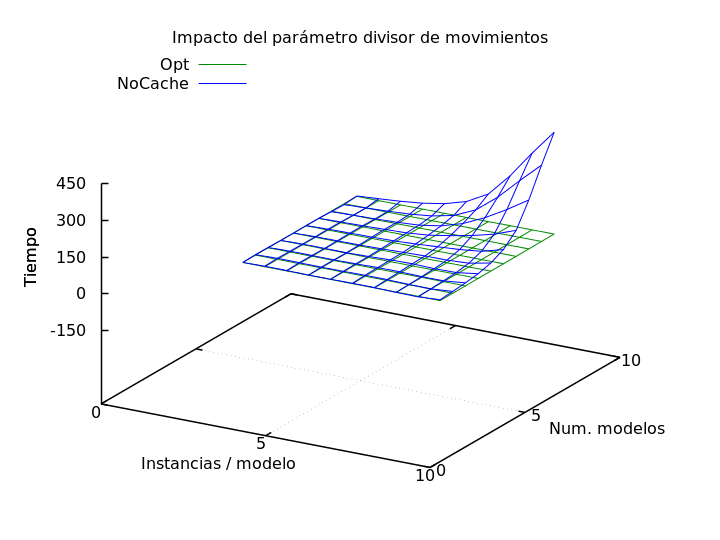
\includegraphics[scale=0.5]{img/comp-nc-opt-spl}
\caption{Gráfica de comparación entre NoCache y ejemplo optimizado
\label{fig:grfcompall}}
\end{figure}






\begin{figure}[H]
\centering
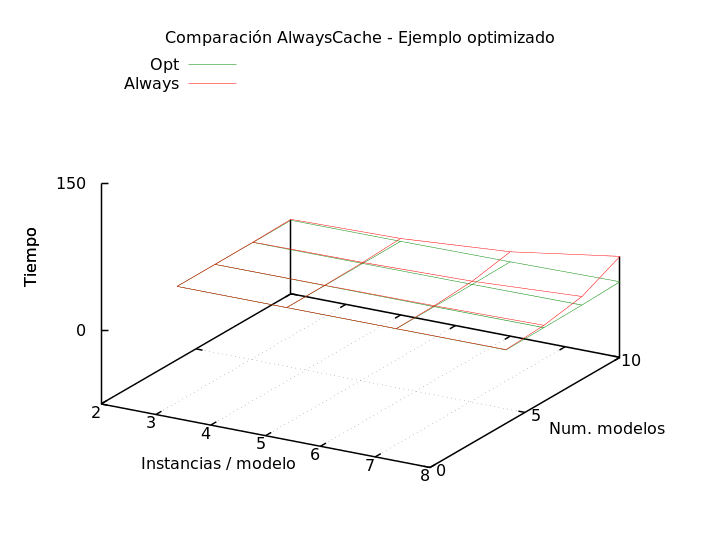
\includegraphics[scale=0.5]{img/comp-alw-opt}
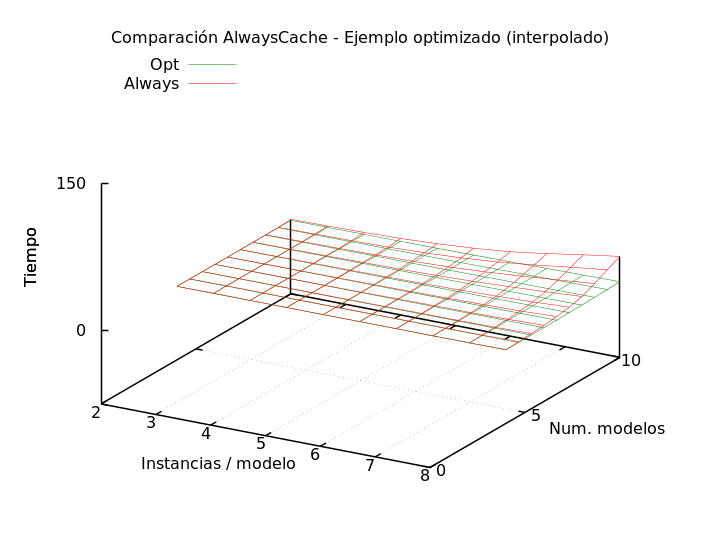
\includegraphics[scale=0.5]{img/comp-alw-opt-spl}
\caption{Gráfica de comparación entre AlwaysCache y ejemplo optimizado
\label{fig:grfcompall}}
\end{figure}








\subsection{Muchos tipos de habitación}

\begin{table}[H]
\begin{center}
	\begin{tabular}{ | c | c | }
\hline
 		Property & Value \\ \hline
DoorGenType & RANDOM \\ 
Refresher cache divisor & 10 \\ 
SolverType & BestSearch \\ 
BestSearch DPE Divisor & 0.9 \\ 
CacheType & REFRESHER \\ 
Random doors param & 0.5 \\ 
\hline
	\end{tabular}
\end{center}
\caption{Configuración test con variabilidad en habitaciones}
\label{table:cfg-optvarsample}
\end{table}


\begin{table}[H]
\begin{center}
	\begin{tabular}{ | c | c | c | c | c | }
\hline
Tam. habs. & Modelos & Instancias/modelo & Total habs. & Tiempo \\ \hline 
6 & 20 & 1 & 20 & 0.0395 \\ 
6 & 20 & 2 & 40 & 0.2505 \\ 
6 & 30 & 1 & 30 & 0.1479 \\ 
6 & 30 & 2 & 60 & 0.9846 \\ 
6 & 40 & 1 & 40 & 0.4307 \\ 
6 & 40 & 2 & 80 & 2.9426 \\ 
6 & 50 & 1 & 50 & 0.9980 \\ 
6 & 50 & 2 & 100 & 7.6388 \\ 
\hline
	\end{tabular}
\end{center}
\caption{Test con variabilidad en habitaciones}
\label{table:optvarsample}
\end{table}


\begin{table}[H]
\begin{center}
	\begin{tabular}{ | c | c | }
\hline
 		Property & Value \\ \hline
DoorGenType & RANDOM \\ 
SolverType & BestSearch \\ 
BestSearch DPE Divisor & 0.5 \\ 
CacheType & ALWAYS \\ 
Random doors param & 0.3 \\ 
\hline
	\end{tabular}
\end{center}
\caption{Configuración para el arreglo del último caso en test con variabilidad en habitaciones}
\label{table:cfg-optvarfix}
\end{table}


\begin{table}[H]
\begin{center}
	\begin{tabular}{ | c | c | c | c | c | }
\hline
Tam. habs. & Modelos & Instancias/modelo & Total habs. & Tiempo \\ \hline 
6 & 20 & 1 & 20 & 0.1615 \\ 
6 & 20 & 2 & 40 & 0.1523 \\ 
6 & 30 & 1 & 30 & 0.0494 \\ 
6 & 30 & 2 & 60 & 0.2139 \\ 
6 & 40 & 1 & 40 & 0.1108 \\ 
6 & 40 & 2 & 80 & 0.6791 \\ 
6 & 50 & 1 & 50 & 0.2222 \\ 
6 & 50 & 2 & 100 & 1.3180 \\ 

\hline
	\end{tabular}
\end{center}
\caption{Arreglo del último caso en test con variabilidad en habitaciones}
\label{table:optvarfix}
\end{table}



